\documentclass[12pt]{article}
% font size could be 10pt (default), 11pt or 12 pt
% paper size coulde be letterpaper (default), legalpaper, executivepaper,
% a4paper, a5paper or b5paper
% side coulde be oneside (default) or twoside 
% columns coulde be onecolumn (default) or twocolumn
% graphics coulde be final (default) or draft 
%
% titlepage coulde be notitlepage (default) or titlepage which 
% makes an extra page for title 
% 
% paper alignment coulde be portrait (default) or landscape 
%
% equations coulde be 
%   default number of the equation on the rigth and equation centered 
%   leqno number on the left and equation centered 
%   fleqn number on the right and  equation on the left side
%
\usepackage{graphicx}
\usepackage{epigraph}
\usepackage{url}
\usepackage{fancybox}
\usepackage{textpos}
\usepackage{indentfirst}
\usepackage{listings}
\usepackage{tcolorbox}
\definecolor{light-gray}{gray}{0.95}
\usepackage{courier}
\lstset{basicstyle=\footnotesize\ttfamily,breaklines=true,numbers=left}
%\usepackage{parskip}
%\setlength{\parskip}{\medskipamount}
\makeatletter
\newcommand{\@minipagerestore}{\setlength{\parskip}{\medskipamount}
\setlength{\parindent}{17pt}}
  \makeatother

\title{Reclaiming a Waveguide Switch -- An Adventure In 3D Printing}
\author{Matt Reilly  \\
	kb1vc \\
	}

\date{\today} 
% \date{\today} date coulde be today 
% \date{25.12.00} or be a certain date
% \date{ } or there is no date 
\begin{document}
% Hint: \title{what ever}, \author{who care} and \date{when ever} could stand 
% before or after the \begin{document} command 
% BUT the \maketitle command MUST come AFTER the \begin{document} command! 
\maketitle

\begin{abstract}
  A simple and somewhat reliable 3D printer can now be had for about \$200.
  While such a printer can help create new widgets and interesting objects, 
  it also affords an opportunity to refurbish or even reclaim equipment that
  may be lying around the shop in need of a hard-to-get part. This is the
  story of one such project that replaced a burned out actuator with a
  R/C model airplane servo and an arduino controller.  All for 
  less than the cost of a replacement unit on eBay.
\end{abstract}

\epigraph{[Engineering] is the art of doing that well with one dollar,
  which any bungler can do with two after a fashion.}{Arthur M. Wellington \\
  ``The Economic Theory of \\
  the Location of Railways''}


%\tableofcontents % create a table of contens 



\section{Introduction}

Most engineers read Mr. Wellington's dictum with great pride
that their training has placed them above the run-of-the-mill bungler.
I know that I do.
When it comes to mechanical engineering, however, I am a bungler.
In this case Wellington provides encouragement: it {\em may} be possible
to do what an expert can do for just twice the cost!

And so began my adventures in 3D printing.


\section{Starting Simple}

This article is about reclaiming a WR75 waveguide switch by adapting
a common hobby airplane servo to function as the positioner. It comprises
a set of plastic parts to couple the servo to the waveguide slug,
and an arduino controller.

But before we dive in to the construction of the waveguide switch positioner,
it may help to look at a much simpler 3D printing project.

Quite a while back, I bought an HP6289A DC power supply at a hamfest.
It was a real find, but at some point in its checkered past it had
been dropped on its face.  The fall shattered the two fine adjustment
knobs.  These were concentric with the coarse adjustment knobs on two
shafts: one for voltage and the second for current.  For years, the
absence of the knobs was no great annoyance. But one night I decided
that making replacements might be a short and simple project.

In the old days, I'd have scavenged in the scrap box for a nylon rod
or perhaps even an aluminum bar, mounted it in the lathe, turned it down,
bored out the hole for the shaft, tracked a few pieces of swarf while
passing through the living room, found that it didn't quite fit, tried
again... In total, I'd have spent a pleasant hour all together from
looking for bar stock, to vacuuming swarf out of the carpet.

This kind of project really points out the virtues of an inexpensive
3D printer.  No great precision is needed, and the cost of a mistake
is a small amount of material and  waiting for the
printer to finish.\footnote{The knobs were very small and simple. They
  took about 15 minutes to print. Typical
  print times for most interesting components can range from one to
  eight hours.}
In fact, it took two tries to get the design right. (Though, had I
been paying attention, it could have been right the first time --
measure twice, print once.) But having the printer in the shack
means that I got through two iterations in less than an hour.
And no metal waste got stuck in the carpet. 


The printer in my shack is a Monoprice Mini Select from \url{https://www.monoprice.com/} shown in Figure \ref{f_printer}.The retail price is \$199. The quality of output from the printer
is variable, but compares favorably with much more expensive printers. Though
the manufacturers claim it can print in a variety of materials, it works best
with PLA, and not at all well with ABS.


\begin{figure}[tb]
  \centering
  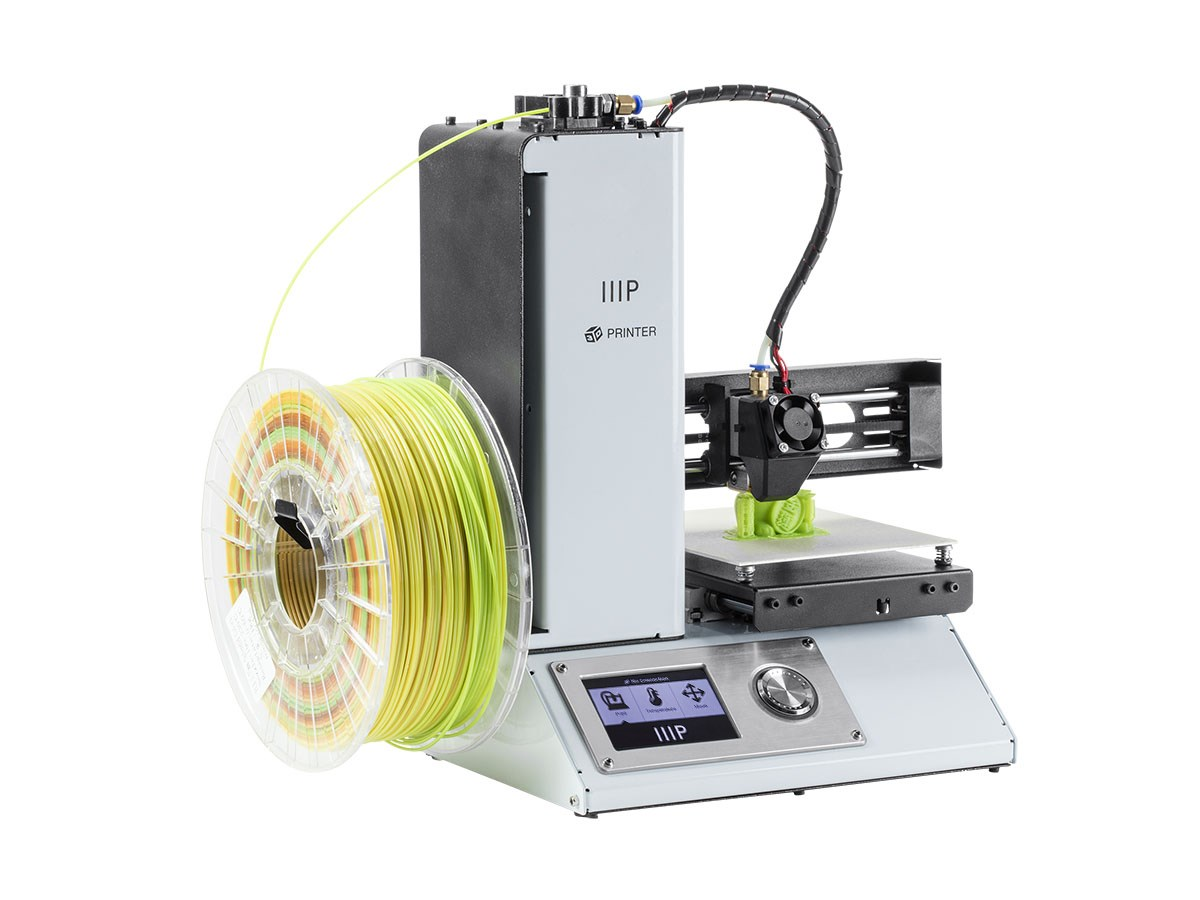
\includegraphics[width=0.6\textwidth]{MiniSelect3DPrinter.jpg}
  \caption{\label{f_printer}The Monoprice Mini Select 3D Printer}
\end{figure}

\begin{figure}[tb]
  %\caption*{About Materials}
\fbox{%
  \begin{minipage}{\textwidth}
\begin{tcolorbox}[colback=gray!35]
    \begin{center}
      {\bf About Materials}
    \end{center}
    ABS (Acrylonitrile Butadiene Styrene, for those keeping score at
    home) is the familiar plastic that shows up in instrument cases,
    helmets, canoes, and waste pipes.  It can be machined, and can
    even be given a glossy finish with exposure to acetone vapors.  It
    is, however, difficult to print on an economy-priced printer.

    PLA (Polylactic Acid) is most often found in disposable drinking
    cups.  It is often used where its potential for recyling is
    important. Some would claim that it is ``biodegradable'' as there
    are bacteria that eat it.  This has caused concern that
    widgets built with PLA might disintegrate while in use.  However,
    the process of breaking down PLA requires a fair amount of
    pressure and/or heat.  Relative durability for PLA can be assured
    by avoiding installations in compost heaps or animals.  Though my
    shack is something of a mess, it has not yet achieved the status
    of ``compost heap.''
    \end{tcolorbox}
\end{minipage}}
\end{figure}

Making the replacement knobs began with a model in OpenSCAD. OpenSCAD
scripts describe three dimensional things by building them
up from simple solids like cubes, spheres, cylinders, and cones.
Shapes can be added or subtracted, so that a simple knob can be
described as an outer cylinder minus an inner cylinder.  The inner
cylinder is the hole for the shaft. OpenSCAD allows the designer to
view an object on screen and to translate scripts into STL (stereo-lithography)
files for later processing. (The description language and the OpenSCAD
editor are described at \url{http://www.openscad.org/}.)

As this project aimed to replace the rather fancy HP original components,
the knobs had a bit of a taper to them, and a hole in the side for a
retaining screw. Figure \ref{f_openscad} is a screenshot of an OpenSCAD
session showing the knob. The model file is shown in Figure \ref{f_knob_list}.

OpenSCAD scripts can follow many forms, but my own approach is to put
all of the important dimensions at the top of the file, and then
describe each feature of the object heirarchically.  For the knobs,
it was useful to describe the shaft diameter (line 2), 
the minimum wall thickness (line 3), the length of the knob (line 5),
the set screw (lines 6 and 7), and the depth of cut for the knurling (line 8).

The knob itself comprises a body, a hole for the shaft, a hole for the
setscrew, and the knurling.  These are all assembled in the last module
{\tt HP6289\_Inner}. The module is actually expanded in lines 39 and 40.
OpenSCAD's default unit is the millimeter, but I tend to measure in
imperial units, so line 39 translates from inches to mm. 

\begin{figure}[tb]
  \centering
  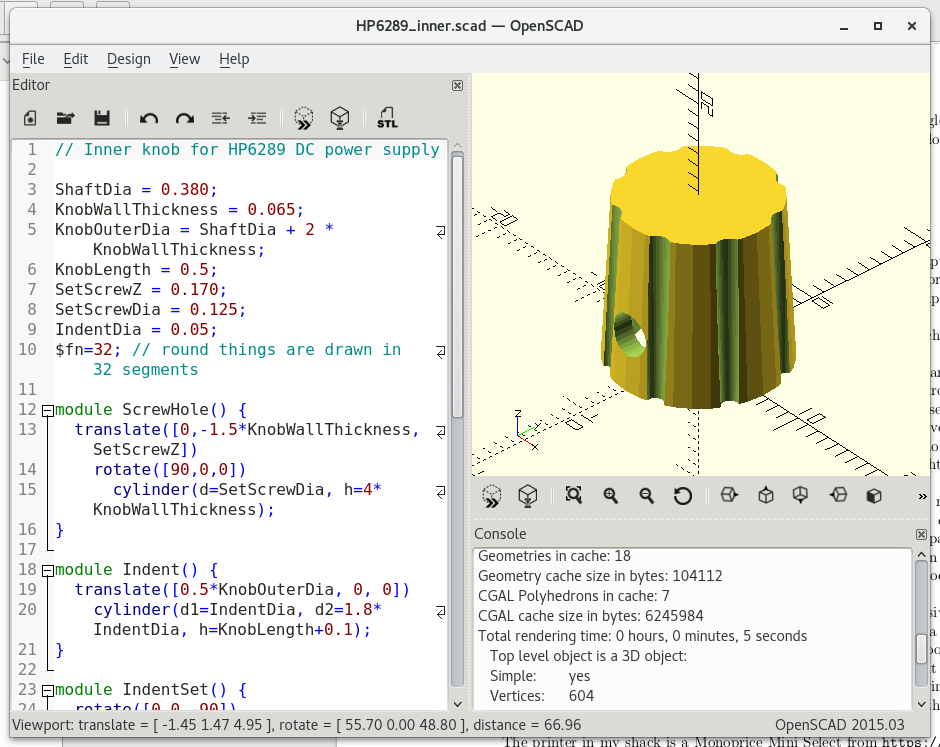
\includegraphics[width=0.6\textwidth]{PSKnob_OpenSCAD.png}
  \caption{\label{f_openscad}OpenSCAD session showing replacement knob}
\end{figure}


\begin{figure}[tb]
\lstinputlisting{HP6289_inner.scad}
\caption{\label{f_knob_list}SCAD description of HP6289 Inner Knobs}
\end{figure}

A pleasant evening of headscratching and printing produced the two knobs
shown in Figure \ref{f_knobs_on_box}.  The result won't be mistaken for
original parts, but the supply is a tool in a workshop, not a museum display. 

\begin{figure}[tb]
  \centering
  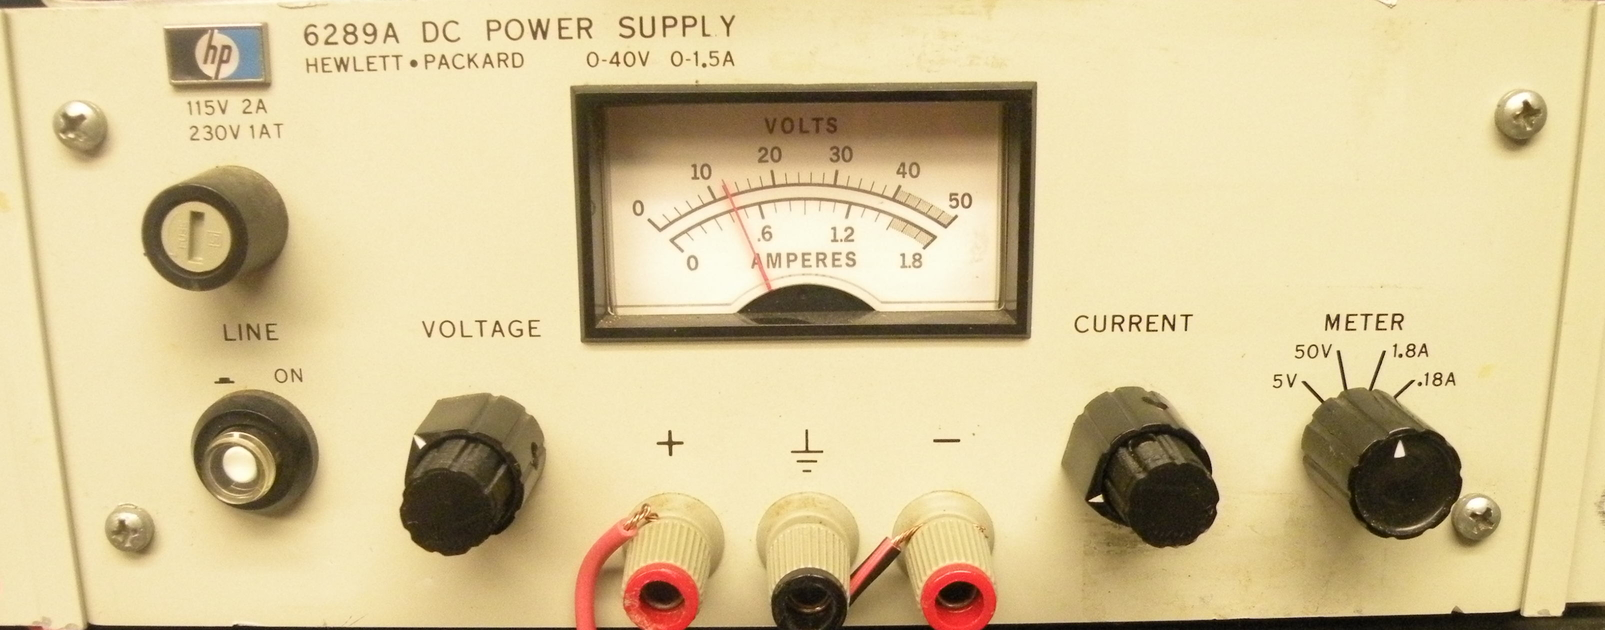
\includegraphics[width=0.8\textwidth]{PSKnobs.jpg}
  \caption{\label{f_knobs_on_box}Replacement power supply knobs in their new home}
\end{figure}

\section{The Waveguide Switch}

Years ago I bought a WR75 waveguide switch to use in a 10GHz transceiver.
The actuator was a pair of coils mounted to a shaft, and surrounded by
a pair of permanent magnets.  The shaft moved a slug inside the switch.
The switch functioned well for about ten years, but finally gasped its last
when one of the coils melted. (It appears that the microswitch that
handled the latching function may have gotten stuck.)

I disassembled the unit to complete the forensic investigation.  A short
examination convinced me that it was toast.  Rewinding the armature was
not all that appealing, and I'd recently acquired some good microwave relays,
so the broken shards sat on the shelf for a year or so, until I found the body
of the switch while looking for something else. The notion hit me that I
could replace the coil/magnet assembly with a R/C model airplane servo.
These were inexpensive and easy to control with an Arduino microcontroller
and a few lines of code.

The trick was mating the servo to the keyed shaft of the waveguide switch,
and sensing the position of the switch.  A typical servo is not very
accurate. The control mechanism is a pulse train where the angular position
of the servo is more-or-less proportional to the pulse width.  The more-or-less
part meant that any positioning mechanism would need some kind of feedback
or other scheme to make sure the waveguide slug was aligned with the input
and output ports.

As an amateur bungler, it took a number of experiments before a reasonably
reliable method for positioning the slug was found. Figure \ref{f_trial_and_error} shows 30 or so parts that were printed on the way to a working design.
The total cost for all the material used in the trials was less than \$10.


\begin{figure}[tb]
  \centering
  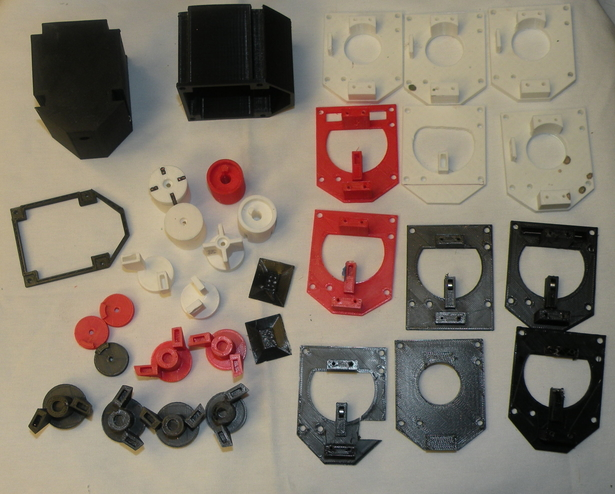
\includegraphics[width=0.8\textwidth]{TrialAndError1.jpg}
  \caption{\label{f_trial_and_error}Trial and Error Parts}
\end{figure}

\begin{figure}[thb]
\centering
    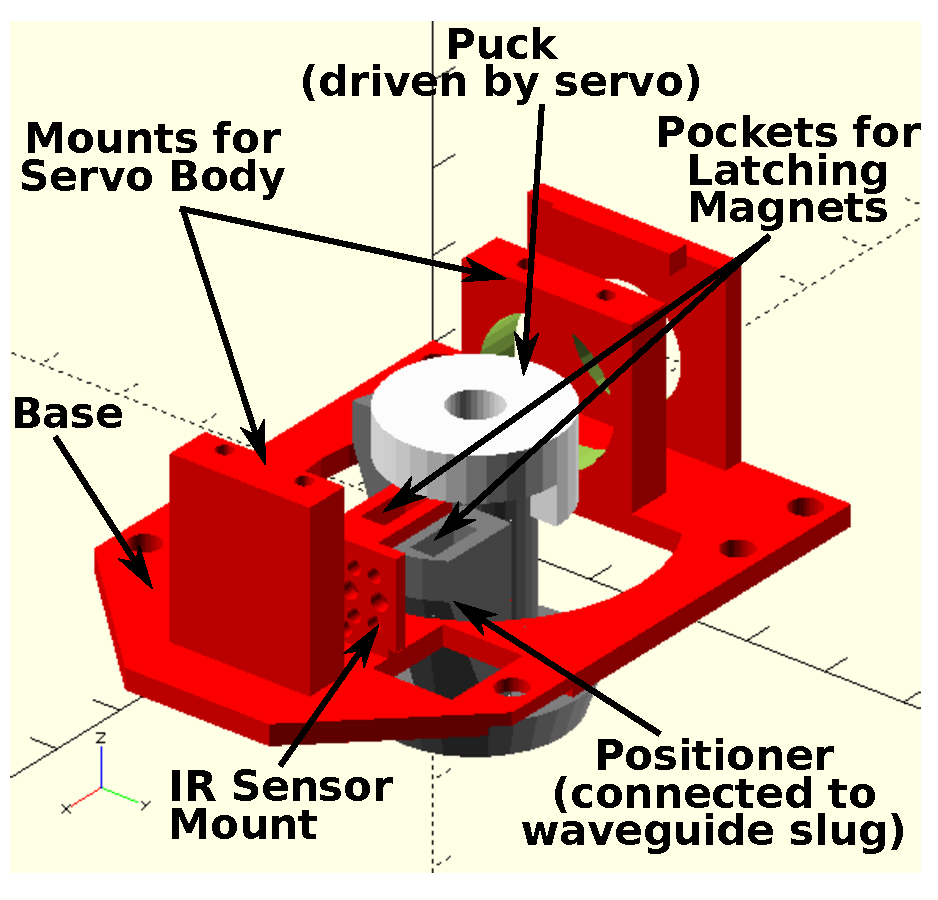
\includegraphics[width=\textwidth]{AssemblyView.pdf}
    \caption{\label{f_expview}The Positioning Mechanism (minus the servo)}  
\end{figure}

Figure \ref{f_wg_switch_orig} shows a switch similar to the unit I started
with.\footnote{Thanks to Dudley Lab \url{http://www.dudleylab.com/surplus6.html}
  for the image.}
%  http://www.dudleylab.com/wr-90-s1.jpg

The ``finished'' unit is shown in Figure \ref{f_wg_switch_new}. 

\begin{figure}[tb]
  \centering
  \begin{minipage}[b]{0.4\textwidth}
    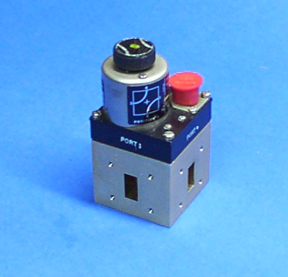
\includegraphics[width=\textwidth]{wr-90-s1.jpg}
    \caption{\label{f_wg_switch_orig}Original switch}  
  \end{minipage}
  \begin{minipage}[b]{0.4\textwidth}
    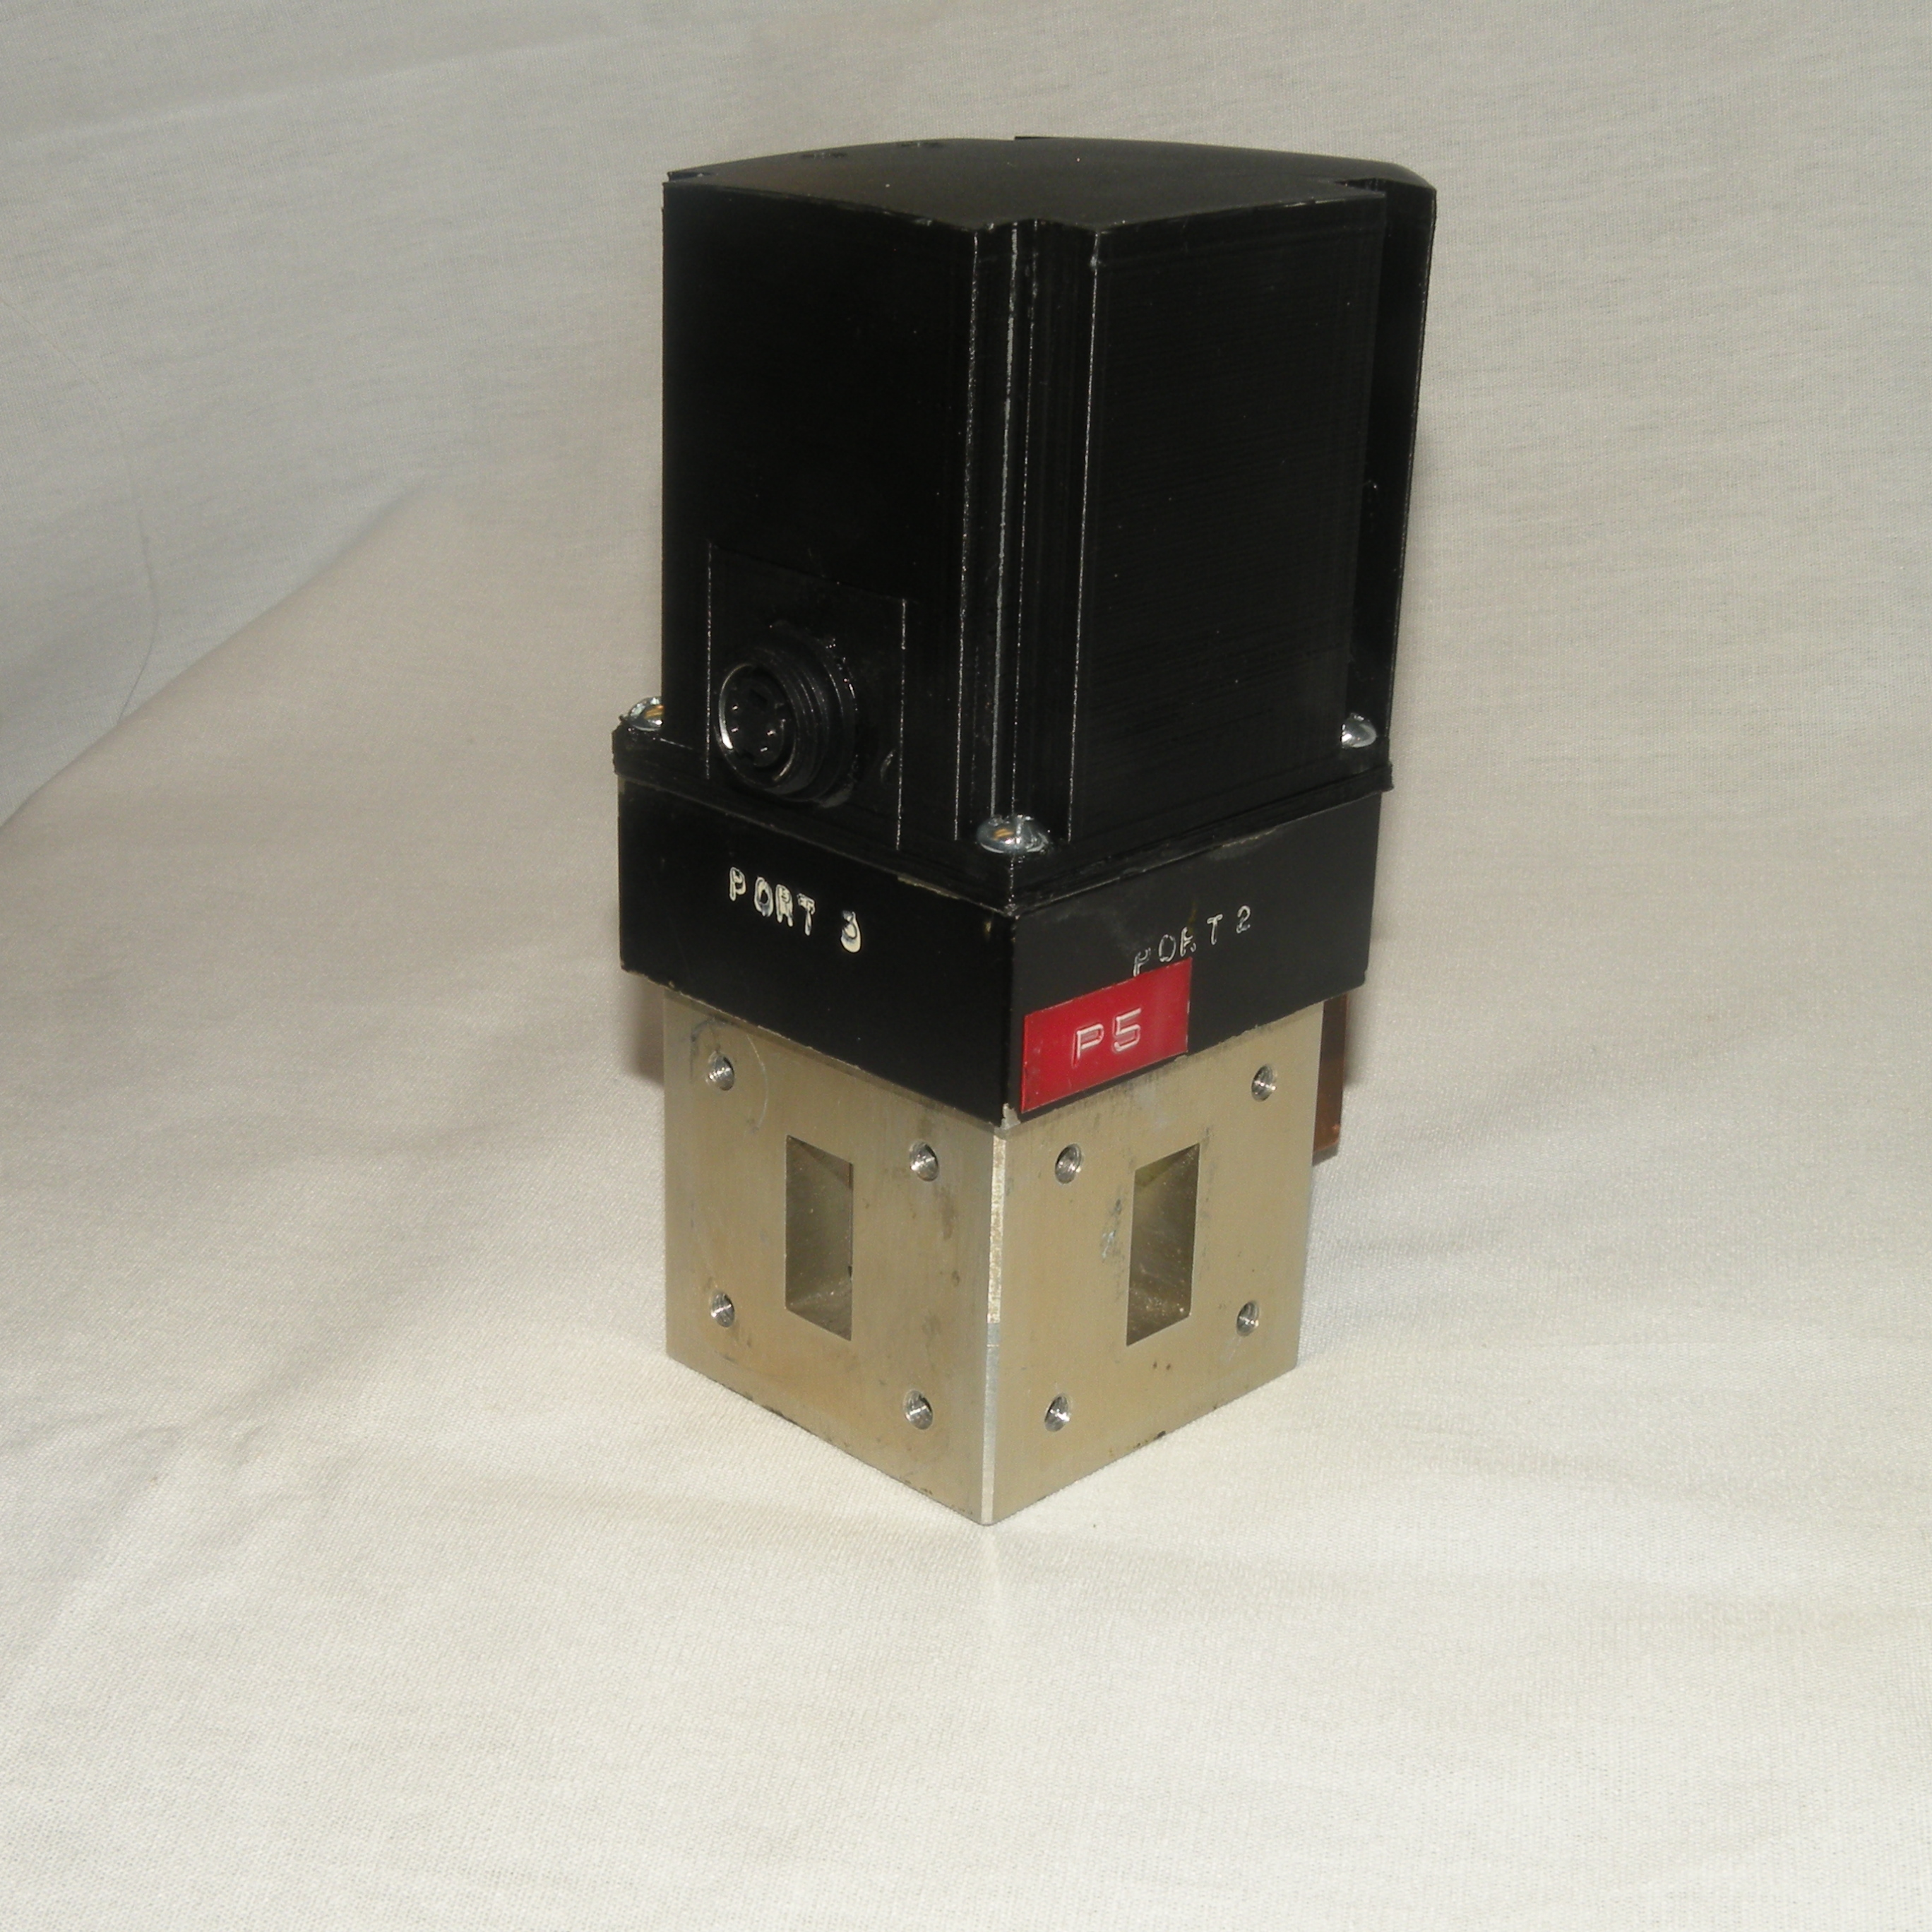
\includegraphics[width=\textwidth]{WGFinal.jpg}
    \caption{\label{f_wg_switch_new}Reclaimed unit)}      
  \end{minipage}
  \end{figure}


\end{document}

